\documentclass[journal,12pt,twocolumn]{IEEEtran}

\usepackage{setspace}
\usepackage{gensymb}

\singlespacing


\usepackage[cmex10]{amsmath}

\usepackage{amsthm}

\usepackage{mathrsfs}
\usepackage{txfonts}
\usepackage{stfloats}
\usepackage{bm}
\usepackage{cite}
\usepackage{cases}
\usepackage{subfig}

\usepackage{longtable}
\usepackage{multirow}

\usepackage{enumitem}
\usepackage{mathtools}
\usepackage{steinmetz}
\usepackage{tikz}
\usepackage{circuitikz}
\usepackage{verbatim}
\usepackage{tfrupee}
\usepackage[breaklinks=true]{hyperref}
\usepackage{graphicx}
\usepackage{tkz-euclide}
\usepackage{float}

\usetikzlibrary{calc,math}
\usepackage{listings}
    \usepackage{color}                                            %%
    \usepackage{array}                                            %%
    \usepackage{longtable}                                        %%
    \usepackage{calc}                                             %%
    \usepackage{multirow}                                         %%
    \usepackage{hhline}                                           %%
    \usepackage{ifthen}                                           %%
    \usepackage{lscape}     
\usepackage{multicol}
\usepackage{chngcntr}

\DeclareMathOperator*{\Res}{Res}

\renewcommand\thesection{\arabic{section}}
\renewcommand\thesubsection{\thesection.\arabic{subsection}}
\renewcommand\thesubsubsection{\thesubsection.\arabic{subsubsection}}

\renewcommand\thesectiondis{\arabic{section}}
\renewcommand\thesubsectiondis{\thesectiondis.\arabic{subsection}}
\renewcommand\thesubsubsectiondis{\thesubsectiondis.\arabic{subsubsection}}


\hyphenation{op-tical net-works semi-conduc-tor}
\def\inputGnumericTable{}                                 %%

\lstset{
%language=C,
frame=single, 
breaklines=true,
columns=fullflexible
}
\begin{document}
\newtheorem{theorem}{Theorem}[section]
\newtheorem{problem}{Problem}
\newtheorem{proposition}{Proposition}[section]
\newtheorem{lemma}{Lemma}[section]
\newtheorem{corollary}[theorem]{Corollary}
\newtheorem{example}{Example}[section]
\newtheorem{definition}[problem]{Definition}

\newcommand{\BEQA}{\begin{eqnarray}}
\newcommand{\EEQA}{\end{eqnarray}}
\newcommand{\define}{\stackrel{\triangle}{=}}
\bibliographystyle{IEEEtran}
\providecommand{\mbf}{\mathbf}
\providecommand{\pr}[1]{\ensuremath{\Pr\left(#1\right)}}
\providecommand{\qfunc}[1]{\ensuremath{Q\left(#1\right)}}
\providecommand{\sbrak}[1]{\ensuremath{{}\left[#1\right]}}
\providecommand{\lsbrak}[1]{\ensuremath{{}\left[#1\right.}}
\providecommand{\rsbrak}[1]{\ensuremath{{}\left.#1\right]}}
\providecommand{\brak}[1]{\ensuremath{\left(#1\right)}}
\providecommand{\lbrak}[1]{\ensuremath{\left(#1\right.}}
\providecommand{\rbrak}[1]{\ensuremath{\left.#1\right)}}
\providecommand{\cbrak}[1]{\ensuremath{\left\{#1\right\}}}
\providecommand{\lcbrak}[1]{\ensuremath{\left\{#1\right.}}
\providecommand{\rcbrak}[1]{\ensuremath{\left.#1\right\}}}
\theoremstyle{remark}
\newtheorem{rem}{Remark}
\newcommand{\sgn}{\mathop{\mathrm{sgn}}}
\providecommand{\abs}[1]{\left\vert#1\right\vert}
\providecommand{\res}[1]{\Res\displaylimits_{#1}} 
\providecommand{\norm}[1]{\left\lVert#1\right\rVert}
%\providecommand{\norm}[1]{\lVert#1\rVert}
\providecommand{\mtx}[1]{\mathbf{#1}}
\providecommand{\mean}[1]{E\left[ #1 \right]}
\providecommand{\fourier}{\overset{\mathcal{F}}{ \rightleftharpoons}}
%\providecommand{\hilbert}{\overset{\mathcal{H}}{ \rightleftharpoons}}
\providecommand{\system}{\overset{\mathcal{H}}{ \longleftrightarrow}}
	%\newcommand{\solution}[2]{\textbf{Solution:}{#1}}
\newcommand{\solution}{\noindent \textbf{Solution: }}
\newcommand{\cosec}{\,\text{cosec}\,}
\providecommand{\dec}[2]{\ensuremath{\overset{#1}{\underset{#2}{\gtrless}}}}
\newcommand{\myvec}[1]{\ensuremath{\begin{pmatrix}#1\end{pmatrix}}}
\newcommand{\mydet}[1]{\ensuremath{\begin{vmatrix}#1\end{vmatrix}}}
\numberwithin{equation}{subsection}
\makeatletter
\@addtoreset{figure}{problem}
\makeatother
\let\StandardTheFigure\thefigure
\let\vec\mathbf
\renewcommand{\thefigure}{\theproblem}
\def\putbox#1#2#3{\makebox[0in][l]{\makebox[#1][l]{}\raisebox{\baselineskip}[0in][0in]{\raisebox{#2}[0in][0in]{#3}}}}
     \def\rightbox#1{\makebox[0in][r]{#1}}
     \def\centbox#1{\makebox[0in]{#1}}
     \def\topbox#1{\raisebox{-\baselineskip}[0in][0in]{#1}}
     \def\midbox#1{\raisebox{-0.5\baselineskip}[0in][0in]{#1}}
\vspace{3cm}
\title{ASSIGNMENT 5}
\author{B.SandhyaRani}
\maketitle
\newpage
\bigskip
\renewcommand{\thefigure}{\theenumi}
\renewcommand{\thetable}{\theenumi}
Download all python codes from 
\begin{lstlisting}
https://github.com/balumurisandhyarani550/Assignment5/tree/main/Assignment5
\end{lstlisting}
%
and latex-tikz codes from 
%
\begin{lstlisting}
https://github.com/balumurisandhyarani550/Assignment5/tree/main/Assignment5
\end{lstlisting}
%
\section{Question No 2.18(Quad forms)}
Find the zero's of the quadratic polynomial $x^2+7x+10$ and verify the relationship between the zero's and the coefficients. 
%
\section{SOLUTION}  
Given
\begin{align}
y& = x^2+7x+10
\\
x^2-y+7x+10 = 0
\end{align}
compare with standard form of equation
\begin{align}
a{x}^2+b{x}{y}+c{y}^2+2d{x}+2e{y}+f = 0
\end{align}
a = 1 , b = 0 , c = 0 , d = $\frac{7}{2}$ , e = $\frac{-1}{2}$ , f = 10
\\
Here,
\begin{align}
\vec{V} = \myvec{1 & 0 \\ 0 & 0},\vec{u}=\myvec{\frac{7}{2}\\ \frac{-1}{2}},f = 10
\\
\abs{V} = \abs{\myvec{1 & 0 \\ 0 & 0}} = 0
\end{align}
\\
Find the eigen values of corresponding $\vec{V}$
\begin{align}
\abs{V-\lambda{I}} = 0
\\
\myvec{1-\lambda & 0 \\ 0 & -\lambda} = 0
\\
\lambda = 0 , 1
\end{align}
$Therefore$ , the corresponding roots are 0 , 1.
\\
Eigen vectors corresponding to $\lambda = 0 , 1$ respectively.
\begin{align}
p_1 = \myvec{0 \\ 1}
\\
p_2 = \myvec{1 \\ 0}
\end{align}
Using eigenvalue decomposition,
\begin{align}
\vec{D} = \myvec{0 & 0\\0 & 1} ,\vec{P}=\myvec{0 & 1\\1 & 0}
\end{align}
Now,
\begin{align}
\myvec{\vec{u}^T + \eta\vec{p_1}^T \\ \vec{V}}\vec{c} &= \myvec{-f \\ \eta\vec{p_1}-\vec{u}} 
\end{align}
$\therefore$Vertex $\vec{c}$ is given by
\begin{align}
\myvec{\frac{7}{2} & -1 \\ 1 & 0 \\ 0 & 0}\vec{c} &= \myvec{-10 \\ \frac{-7}{2} \\ 0} \\
\implies  \myvec{\frac{7}{2} & -1 \\ 1 & 0}\vec{c} &= \myvec{-10 \\ \frac{-7}{2}}
\\
\implies \vec{c} &= \myvec{\frac{-7}{2}\\\frac{-9}{4}}
\end{align}
\numberwithin{figure}{section}
\begin{figure}[!ht]
\centering
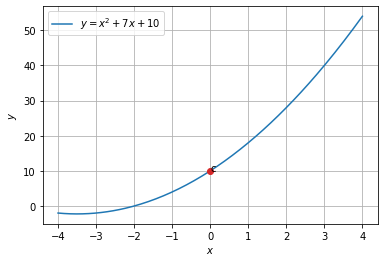
\includegraphics[width=\columnwidth]{download.png}
\caption{$y=x^2+7x+10$}
\label{ex3}	
\end{figure}
Now,
\begin{align}
\vec{p_1}^T\vec{c} &= \myvec{0 & 1}\myvec{\frac{-7}{2}\\\frac{-9}{4}}
\\
&= \frac{-9}{4}
\end{align}
and,
\begin{align}
\vec{p_2}^T\vec{V}\vec{p_2} &= \myvec{1 & 0}\myvec{1 & 0\\0& 0}\myvec{1 \\ 0}
\\
&= 1
\end{align}
$\because$
\begin{align}
(\vec{p_1}^T\vec{c})(\vec{p_2}^T\vec{V}\vec{p_2}) = \frac{-9}{4}<0
\end{align}
Hence,the given equation has real roots.
\end{document}